% Options for packages loaded elsewhere
\PassOptionsToPackage{unicode}{hyperref}
\PassOptionsToPackage{hyphens}{url}
%
\documentclass[
]{article}
\usepackage{amsmath,amssymb}
\usepackage{iftex}
\ifPDFTeX
  \usepackage[T1]{fontenc}
  \usepackage[utf8]{inputenc}
  \usepackage{textcomp} % provide euro and other symbols
\else % if luatex or xetex
  \usepackage{unicode-math} % this also loads fontspec
  \defaultfontfeatures{Scale=MatchLowercase}
  \defaultfontfeatures[\rmfamily]{Ligatures=TeX,Scale=1}
\fi
\usepackage{lmodern}
\ifPDFTeX\else
  % xetex/luatex font selection
\fi
% Use upquote if available, for straight quotes in verbatim environments
\IfFileExists{upquote.sty}{\usepackage{upquote}}{}
\IfFileExists{microtype.sty}{% use microtype if available
  \usepackage[]{microtype}
  \UseMicrotypeSet[protrusion]{basicmath} % disable protrusion for tt fonts
}{}
\makeatletter
\@ifundefined{KOMAClassName}{% if non-KOMA class
  \IfFileExists{parskip.sty}{%
    \usepackage{parskip}
  }{% else
    \setlength{\parindent}{0pt}
    \setlength{\parskip}{6pt plus 2pt minus 1pt}}
}{% if KOMA class
  \KOMAoptions{parskip=half}}
\makeatother
\usepackage{xcolor}
\usepackage[margin=1in]{geometry}
\usepackage{color}
\usepackage{fancyvrb}
\newcommand{\VerbBar}{|}
\newcommand{\VERB}{\Verb[commandchars=\\\{\}]}
\DefineVerbatimEnvironment{Highlighting}{Verbatim}{commandchars=\\\{\}}
% Add ',fontsize=\small' for more characters per line
\usepackage{framed}
\definecolor{shadecolor}{RGB}{248,248,248}
\newenvironment{Shaded}{\begin{snugshade}}{\end{snugshade}}
\newcommand{\AlertTok}[1]{\textcolor[rgb]{0.94,0.16,0.16}{#1}}
\newcommand{\AnnotationTok}[1]{\textcolor[rgb]{0.56,0.35,0.01}{\textbf{\textit{#1}}}}
\newcommand{\AttributeTok}[1]{\textcolor[rgb]{0.13,0.29,0.53}{#1}}
\newcommand{\BaseNTok}[1]{\textcolor[rgb]{0.00,0.00,0.81}{#1}}
\newcommand{\BuiltInTok}[1]{#1}
\newcommand{\CharTok}[1]{\textcolor[rgb]{0.31,0.60,0.02}{#1}}
\newcommand{\CommentTok}[1]{\textcolor[rgb]{0.56,0.35,0.01}{\textit{#1}}}
\newcommand{\CommentVarTok}[1]{\textcolor[rgb]{0.56,0.35,0.01}{\textbf{\textit{#1}}}}
\newcommand{\ConstantTok}[1]{\textcolor[rgb]{0.56,0.35,0.01}{#1}}
\newcommand{\ControlFlowTok}[1]{\textcolor[rgb]{0.13,0.29,0.53}{\textbf{#1}}}
\newcommand{\DataTypeTok}[1]{\textcolor[rgb]{0.13,0.29,0.53}{#1}}
\newcommand{\DecValTok}[1]{\textcolor[rgb]{0.00,0.00,0.81}{#1}}
\newcommand{\DocumentationTok}[1]{\textcolor[rgb]{0.56,0.35,0.01}{\textbf{\textit{#1}}}}
\newcommand{\ErrorTok}[1]{\textcolor[rgb]{0.64,0.00,0.00}{\textbf{#1}}}
\newcommand{\ExtensionTok}[1]{#1}
\newcommand{\FloatTok}[1]{\textcolor[rgb]{0.00,0.00,0.81}{#1}}
\newcommand{\FunctionTok}[1]{\textcolor[rgb]{0.13,0.29,0.53}{\textbf{#1}}}
\newcommand{\ImportTok}[1]{#1}
\newcommand{\InformationTok}[1]{\textcolor[rgb]{0.56,0.35,0.01}{\textbf{\textit{#1}}}}
\newcommand{\KeywordTok}[1]{\textcolor[rgb]{0.13,0.29,0.53}{\textbf{#1}}}
\newcommand{\NormalTok}[1]{#1}
\newcommand{\OperatorTok}[1]{\textcolor[rgb]{0.81,0.36,0.00}{\textbf{#1}}}
\newcommand{\OtherTok}[1]{\textcolor[rgb]{0.56,0.35,0.01}{#1}}
\newcommand{\PreprocessorTok}[1]{\textcolor[rgb]{0.56,0.35,0.01}{\textit{#1}}}
\newcommand{\RegionMarkerTok}[1]{#1}
\newcommand{\SpecialCharTok}[1]{\textcolor[rgb]{0.81,0.36,0.00}{\textbf{#1}}}
\newcommand{\SpecialStringTok}[1]{\textcolor[rgb]{0.31,0.60,0.02}{#1}}
\newcommand{\StringTok}[1]{\textcolor[rgb]{0.31,0.60,0.02}{#1}}
\newcommand{\VariableTok}[1]{\textcolor[rgb]{0.00,0.00,0.00}{#1}}
\newcommand{\VerbatimStringTok}[1]{\textcolor[rgb]{0.31,0.60,0.02}{#1}}
\newcommand{\WarningTok}[1]{\textcolor[rgb]{0.56,0.35,0.01}{\textbf{\textit{#1}}}}
\usepackage{graphicx}
\makeatletter
\def\maxwidth{\ifdim\Gin@nat@width>\linewidth\linewidth\else\Gin@nat@width\fi}
\def\maxheight{\ifdim\Gin@nat@height>\textheight\textheight\else\Gin@nat@height\fi}
\makeatother
% Scale images if necessary, so that they will not overflow the page
% margins by default, and it is still possible to overwrite the defaults
% using explicit options in \includegraphics[width, height, ...]{}
\setkeys{Gin}{width=\maxwidth,height=\maxheight,keepaspectratio}
% Set default figure placement to htbp
\makeatletter
\def\fps@figure{htbp}
\makeatother
\setlength{\emergencystretch}{3em} % prevent overfull lines
\providecommand{\tightlist}{%
  \setlength{\itemsep}{0pt}\setlength{\parskip}{0pt}}
\setcounter{secnumdepth}{-\maxdimen} % remove section numbering
\usepackage{fontspec}
\setmainfont{Times New Roman}
\usepackage{ctex}
\ifLuaTeX
  \usepackage{selnolig}  % disable illegal ligatures
\fi
\usepackage{bookmark}
\IfFileExists{xurl.sty}{\usepackage{xurl}}{} % add URL line breaks if available
\urlstyle{same}
\hypersetup{
  pdftitle={homework2},
  pdfauthor={黄舟翔 3220103606},
  hidelinks,
  pdfcreator={LaTeX via pandoc}}

\title{homework2}
\author{黄舟翔 3220103606}
\date{2025-06-27}

\begin{document}
\maketitle

The data set calif\_penn\_2011.csv contains information about the
housing stock of California and Pennsylvania, as of 2011. Information as
aggregated into ``Census tracts'', geographic regions of a few thousand
people which are supposed to be fairly homogeneous economically and
socially.

\subsubsection{\texorpdfstring{1. \emph{Loading and
cleaning}}{1. Loading and cleaning}}\label{loading-and-cleaning}

\paragraph{a.}\label{a.}

Load the data into a dataframe called \texttt{ca\_pa}.

\begin{Shaded}
\begin{Highlighting}[]
\FunctionTok{library}\NormalTok{(tidyverse)}
\NormalTok{ca\_pa }\OtherTok{\textless{}{-}} \FunctionTok{read.csv}\NormalTok{(}\StringTok{"data/calif\_penn\_2011.csv"}\NormalTok{)}
\end{Highlighting}
\end{Shaded}

\paragraph{b.}\label{b.}

How many rows and columns does the dataframe have?

\begin{Shaded}
\begin{Highlighting}[]
\FunctionTok{cat}\NormalTok{(}\StringTok{"原始数据维度:"}\NormalTok{, }\FunctionTok{nrow}\NormalTok{(ca\_pa), }\StringTok{"行 ×"}\NormalTok{, }\FunctionTok{ncol}\NormalTok{(ca\_pa), }\StringTok{"列}\SpecialCharTok{\textbackslash{}n}\StringTok{"}\NormalTok{)}
\end{Highlighting}
\end{Shaded}

\begin{verbatim}
## 原始数据维度: 11275 行 × 34 列
\end{verbatim}

\paragraph{c.~}\label{c.}

Run this command, and explain, in words, what this does:

该代码是在完成每列缺失值数量的统计。

\begin{Shaded}
\begin{Highlighting}[]
\NormalTok{na\_counts }\OtherTok{\textless{}{-}} \FunctionTok{colSums}\NormalTok{(}\FunctionTok{apply}\NormalTok{(ca\_pa,}\FunctionTok{c}\NormalTok{(}\DecValTok{1}\NormalTok{,}\DecValTok{2}\NormalTok{),is.na))}
\FunctionTok{cat}\NormalTok{(}\StringTok{"}\SpecialCharTok{\textbackslash{}n}\StringTok{每列缺失值统计:}\SpecialCharTok{\textbackslash{}n}\StringTok{"}\NormalTok{)}
\end{Highlighting}
\end{Shaded}

\begin{verbatim}
## 
## 每列缺失值统计:
\end{verbatim}

\begin{Shaded}
\begin{Highlighting}[]
\FunctionTok{print}\NormalTok{(na\_counts)}
\end{Highlighting}
\end{Shaded}

\begin{verbatim}
##                           X                     GEO.id2 
##                           0                           0 
##                     STATEFP                    COUNTYFP 
##                           0                           0 
##                     TRACTCE                  POPULATION 
##                           0                           0 
##                    LATITUDE                   LONGITUDE 
##                           0                           0 
##           GEO.display.label          Median_house_value 
##                           0                         599 
##                 Total_units                Vacant_units 
##                           0                           0 
##                Median_rooms  Mean_household_size_owners 
##                         157                         215 
## Mean_household_size_renters         Built_2005_or_later 
##                         152                          98 
##          Built_2000_to_2004                 Built_1990s 
##                          98                          98 
##                 Built_1980s                 Built_1970s 
##                          98                          98 
##                 Built_1960s                 Built_1950s 
##                          98                          98 
##                 Built_1940s       Built_1939_or_earlier 
##                          98                          98 
##                  Bedrooms_0                  Bedrooms_1 
##                          98                          98 
##                  Bedrooms_2                  Bedrooms_3 
##                          98                          98 
##                  Bedrooms_4          Bedrooms_5_or_more 
##                          98                          98 
##                      Owners                     Renters 
##                         100                         100 
##     Median_household_income       Mean_household_income 
##                         115                         126
\end{verbatim}

\paragraph{d.}\label{d.}

The function \texttt{na.omit()} takes a dataframe and returns a new
dataframe, omitting any row containing an NA value. Use it to purge the
data set of rows with incomplete data.

\begin{Shaded}
\begin{Highlighting}[]
\NormalTok{      ca\_pa\_clean }\OtherTok{\textless{}{-}} \FunctionTok{na.omit}\NormalTok{(ca\_pa)}
\end{Highlighting}
\end{Shaded}

\paragraph{e.}\label{e.}

How many rows did this eliminate?

\begin{Shaded}
\begin{Highlighting}[]
\NormalTok{rows\_eliminated }\OtherTok{\textless{}{-}} \FunctionTok{nrow}\NormalTok{(ca\_pa) }\SpecialCharTok{{-}} \FunctionTok{nrow}\NormalTok{(ca\_pa\_clean)}
\FunctionTok{cat}\NormalTok{(}\StringTok{"}\SpecialCharTok{\textbackslash{}n}\StringTok{删除的行数:"}\NormalTok{, rows\_eliminated)}
\end{Highlighting}
\end{Shaded}

\begin{verbatim}
## 
## 删除的行数: 670
\end{verbatim}

\paragraph{f.}\label{f.}

Are your answers in (c) and (e) compatible? Explain.

是兼容的:na.omit()删除包含任意NA的整行

理论删除行数 = (所有列NA总数之和)/列数

实际因每行可能有多个NA,但删除行数应与NA分布一致

\subsubsection{\texorpdfstring{2.\emph{This Very New
House}}{2.This Very New House}}\label{this-very-new-house}

\paragraph{a.}\label{a.-1}

The variable \texttt{Built\_2005\_or\_later} indicates the percentage of
houses in each Census tract built since 2005. Plot median house prices
against this variable.

可以用下列代码解决问题

\begin{Shaded}
\begin{Highlighting}[]
\NormalTok{p1 }\OtherTok{\textless{}{-}} \FunctionTok{ggplot}\NormalTok{(ca\_pa\_clean, }\FunctionTok{aes}\NormalTok{(}\AttributeTok{x =}\NormalTok{ Built\_2005\_or\_later, }\AttributeTok{y =}\NormalTok{ Median\_house\_value)) }\SpecialCharTok{+}
  \FunctionTok{geom\_point}\NormalTok{(}\AttributeTok{alpha =} \FloatTok{0.4}\NormalTok{, }\AttributeTok{color =} \StringTok{"steelblue"}\NormalTok{) }\SpecialCharTok{+}
  \FunctionTok{labs}\NormalTok{(}\AttributeTok{title =} \StringTok{"New Houses vs. House Value"}\NormalTok{,}
       \AttributeTok{x =} \StringTok{"Houses Built Since 2005 (\%)"}\NormalTok{, }
       \AttributeTok{y =} \StringTok{"Median House Value"}\NormalTok{) }\SpecialCharTok{+}
  \FunctionTok{theme\_minimal}\NormalTok{() }\SpecialCharTok{+}
  \FunctionTok{theme}\NormalTok{(}\AttributeTok{plot.title =} \FunctionTok{element\_text}\NormalTok{(}\AttributeTok{hjust =} \FloatTok{0.5}\NormalTok{),}
        \AttributeTok{plot.margin =} \FunctionTok{margin}\NormalTok{(}\AttributeTok{t=}\DecValTok{10}\NormalTok{, }\AttributeTok{r=}\DecValTok{10}\NormalTok{, }\AttributeTok{b=}\DecValTok{10}\NormalTok{, }\AttributeTok{l=}\DecValTok{10}\NormalTok{, }\AttributeTok{unit=}\StringTok{"pt"}\NormalTok{))}
\FunctionTok{print}\NormalTok{(p1)}
\end{Highlighting}
\end{Shaded}

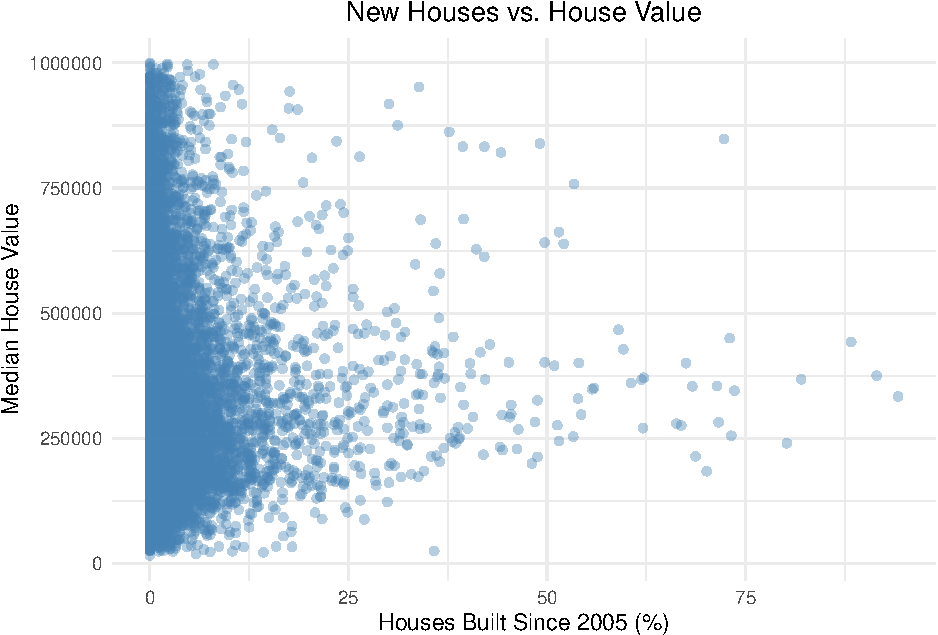
\includegraphics{Homework-02_files/figure-latex/unnamed-chunk-6-1.pdf}

\paragraph{b.}\label{b.-1}

Make a new plot, or pair of plots, which breaks this out by state. Note
that the state is recorded in the \texttt{STATEFP} variable, with
California being state 6 and Pennsylvania state 42.

可以用下列代码解决

\begin{Shaded}
\begin{Highlighting}[]
\NormalTok{ca\_pa\_clean }\OtherTok{\textless{}{-}}\NormalTok{ ca\_pa\_clean }\SpecialCharTok{\%\textgreater{}\%}
  \FunctionTok{mutate}\NormalTok{(}\AttributeTok{State =} \FunctionTok{ifelse}\NormalTok{(STATEFP }\SpecialCharTok{==} \DecValTok{6}\NormalTok{, }\StringTok{"California"}\NormalTok{,}
                        \FunctionTok{ifelse}\NormalTok{(STATEFP }\SpecialCharTok{==} \DecValTok{42}\NormalTok{, }\StringTok{"Pennsylvania"}\NormalTok{, }\StringTok{"Other"}\NormalTok{)))}
\NormalTok{p2 }\OtherTok{\textless{}{-}} \FunctionTok{ggplot}\NormalTok{(ca\_pa\_clean, }\FunctionTok{aes}\NormalTok{(}\AttributeTok{x =}\NormalTok{ Built\_2005\_or\_later, }
  \AttributeTok{y =}\NormalTok{ Median\_house\_value, }\AttributeTok{color =}\NormalTok{ State)) }\SpecialCharTok{+}
  \FunctionTok{geom\_point}\NormalTok{(}\AttributeTok{alpha =} \FloatTok{0.4}\NormalTok{) }\SpecialCharTok{+}
  \FunctionTok{scale\_color\_manual}\NormalTok{(}\AttributeTok{values =} \FunctionTok{c}\NormalTok{(}\StringTok{"California"} \OtherTok{=} \StringTok{"red"}\NormalTok{, }\StringTok{"Pennsylvania"} \OtherTok{=} \StringTok{"blue"}\NormalTok{)) }\SpecialCharTok{+}
  \FunctionTok{facet\_wrap}\NormalTok{(}\SpecialCharTok{\textasciitilde{}}\NormalTok{State, }\AttributeTok{scales =} \StringTok{"free"}\NormalTok{) }\SpecialCharTok{+}
  \FunctionTok{labs}\NormalTok{(}\AttributeTok{title =} \StringTok{"New Houses vs. House Value by State"}\NormalTok{,}
       \AttributeTok{x =} \StringTok{"Houses Built Since 2005 (\%)"}\NormalTok{, }
       \AttributeTok{y =} \StringTok{"Median House Value"}\NormalTok{) }\SpecialCharTok{+}
  \FunctionTok{theme\_minimal}\NormalTok{() }\SpecialCharTok{+}
  \FunctionTok{theme}\NormalTok{(}\AttributeTok{legend.position =} \StringTok{"none"}\NormalTok{,}
        \AttributeTok{plot.title =} \FunctionTok{element\_text}\NormalTok{(}\AttributeTok{hjust =} \FloatTok{0.5}\NormalTok{),}
        \AttributeTok{plot.margin =} \FunctionTok{margin}\NormalTok{(}\AttributeTok{t=}\DecValTok{10}\NormalTok{, }\AttributeTok{r=}\DecValTok{10}\NormalTok{, }\AttributeTok{b=}\DecValTok{10}\NormalTok{, }\AttributeTok{l=}\DecValTok{10}\NormalTok{, }\AttributeTok{unit=}\StringTok{"pt"}\NormalTok{))}
\FunctionTok{print}\NormalTok{(p2)}
\end{Highlighting}
\end{Shaded}

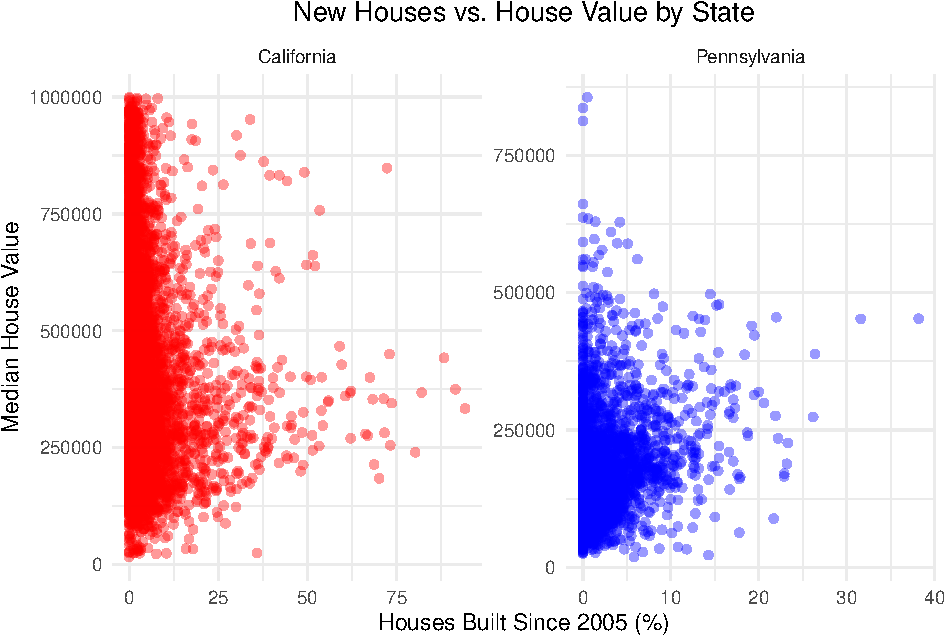
\includegraphics{Homework-02_files/figure-latex/unnamed-chunk-7-1.pdf}

\subsubsection{\texorpdfstring{3. \emph{Nobody
Home}}{3. Nobody Home}}\label{nobody-home}

The vacancy rate is the fraction of housing units which are not
occupied. The dataframe contains columns giving the total number of
housing units for each Census tract, and the number of vacant housing
units.

\paragraph{a.}\label{a.-2}

Add a new column to the dataframe which contains the vacancy rate. What
are the minimum, maximum, mean, and median vacancy rates?

可以用以下代码完成:

\begin{Shaded}
\begin{Highlighting}[]
\NormalTok{ca\_pa\_clean }\OtherTok{\textless{}{-}}\NormalTok{ ca\_pa\_clean }\SpecialCharTok{\%\textgreater{}\%}
  \FunctionTok{mutate}\NormalTok{(}\AttributeTok{Vacancy\_Rate =}\NormalTok{ Vacant\_units }\SpecialCharTok{/}\NormalTok{ Total\_units)}

\NormalTok{vacancy\_stats }\OtherTok{\textless{}{-}} \FunctionTok{summary}\NormalTok{(ca\_pa\_clean}\SpecialCharTok{$}\NormalTok{Vacancy\_Rate)}
\FunctionTok{print}\NormalTok{(vacancy\_stats)}
\end{Highlighting}
\end{Shaded}

\begin{verbatim}
##    Min. 1st Qu.  Median    Mean 3rd Qu.    Max. 
## 0.00000 0.03846 0.06767 0.08889 0.10921 0.96531
\end{verbatim}

\paragraph{b.}\label{b.-2}

Plot the vacancy rate against median house value.

可以用以下代码完成:

\begin{Shaded}
\begin{Highlighting}[]
\NormalTok{p3 }\OtherTok{\textless{}{-}} \FunctionTok{ggplot}\NormalTok{(ca\_pa\_clean, }\FunctionTok{aes}\NormalTok{(}\AttributeTok{x =}\NormalTok{ Vacancy\_Rate, }\AttributeTok{y =}\NormalTok{ Median\_house\_value)) }\SpecialCharTok{+}
  \FunctionTok{geom\_point}\NormalTok{(}\AttributeTok{alpha =} \FloatTok{0.3}\NormalTok{, }\AttributeTok{color =} \StringTok{"darkgreen"}\NormalTok{) }\SpecialCharTok{+}
  \FunctionTok{geom\_smooth}\NormalTok{(}\AttributeTok{method =} \StringTok{"lm"}\NormalTok{, }\AttributeTok{color =} \StringTok{"red"}\NormalTok{, }\AttributeTok{se =} \ConstantTok{FALSE}\NormalTok{) }\SpecialCharTok{+}
  \FunctionTok{labs}\NormalTok{(}\AttributeTok{title =} \StringTok{"Vacancy Rate vs. House Value"}\NormalTok{,}
       \AttributeTok{x =} \StringTok{"Vacancy Rate"}\NormalTok{, }
       \AttributeTok{y =} \StringTok{"Median House Value"}\NormalTok{) }\SpecialCharTok{+}
  \FunctionTok{theme\_minimal}\NormalTok{() }\SpecialCharTok{+}
  \FunctionTok{theme}\NormalTok{(}\AttributeTok{plot.title =} \FunctionTok{element\_text}\NormalTok{(}\AttributeTok{hjust =} \FloatTok{0.5}\NormalTok{),}
        \AttributeTok{plot.margin =} \FunctionTok{margin}\NormalTok{(}\DecValTok{10}\NormalTok{, }\DecValTok{10}\NormalTok{, }\DecValTok{10}\NormalTok{, }\DecValTok{10}\NormalTok{))}
\FunctionTok{print}\NormalTok{(p3)}
\end{Highlighting}
\end{Shaded}

\begin{verbatim}
## `geom_smooth()` using formula = 'y ~ x'
\end{verbatim}

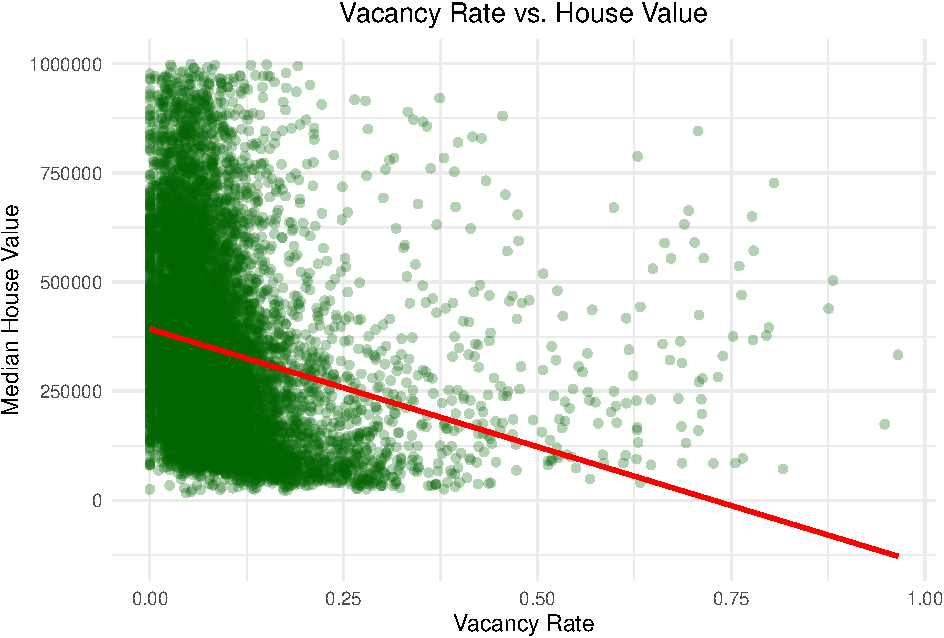
\includegraphics{Homework-02_files/figure-latex/unnamed-chunk-9-1.pdf}

\paragraph{c.}\label{c.-1}

Plot vacancy rate against median house value separately for California
and for Pennsylvania. Is there a difference?

可以用下列代码完成

\begin{Shaded}
\begin{Highlighting}[]
\NormalTok{ca\_pa\_clean }\OtherTok{\textless{}{-}}\NormalTok{ ca\_pa\_clean }\SpecialCharTok{\%\textgreater{}\%}
  \FunctionTok{mutate}\NormalTok{(}\AttributeTok{state =} \FunctionTok{case\_when}\NormalTok{(}
\NormalTok{    STATEFP }\SpecialCharTok{==} \DecValTok{6} \SpecialCharTok{\textasciitilde{}} \StringTok{"California"}\NormalTok{,}
\NormalTok{    STATEFP }\SpecialCharTok{==} \DecValTok{42} \SpecialCharTok{\textasciitilde{}} \StringTok{"Pennsylvania"}\NormalTok{,}
    \ConstantTok{TRUE} \SpecialCharTok{\textasciitilde{}} \StringTok{"Other"}
\NormalTok{  )) }\SpecialCharTok{\%\textgreater{}\%}
  \FunctionTok{filter}\NormalTok{(state }\SpecialCharTok{!=} \StringTok{"Other"}\NormalTok{)  }\CommentTok{\# 仅保留两个州的数据}

\CommentTok{\# 分面散点图}
\FunctionTok{ggplot}\NormalTok{(ca\_pa\_clean, }\FunctionTok{aes}\NormalTok{(}\AttributeTok{y =}\NormalTok{ Median\_house\_value, }\AttributeTok{x =}\NormalTok{ Vacancy\_Rate)) }\SpecialCharTok{+}
  \FunctionTok{geom\_point}\NormalTok{(}\FunctionTok{aes}\NormalTok{(}\AttributeTok{color =}\NormalTok{ state), }\AttributeTok{alpha =} \FloatTok{0.7}\NormalTok{, }\AttributeTok{size =} \DecValTok{2}\NormalTok{) }\SpecialCharTok{+}
  \FunctionTok{geom\_smooth}\NormalTok{(}\FunctionTok{aes}\NormalTok{(}\AttributeTok{color =}\NormalTok{ state), }\AttributeTok{method =} \StringTok{"loess"}\NormalTok{, }\AttributeTok{se =} \ConstantTok{FALSE}\NormalTok{) }\SpecialCharTok{+}
  \FunctionTok{facet\_wrap}\NormalTok{(}\SpecialCharTok{\textasciitilde{}}\NormalTok{state, }\AttributeTok{scales =} \StringTok{"free\_x"}\NormalTok{) }\SpecialCharTok{+}  
  \FunctionTok{scale\_color\_manual}\NormalTok{(}\AttributeTok{values =} \FunctionTok{c}\NormalTok{(}\StringTok{"California"} \OtherTok{=} \StringTok{"\#E74C3C"}\NormalTok{, }
                                \StringTok{"Pennsylvania"} \OtherTok{=} \StringTok{"\#2980B9"}\NormalTok{)) }\SpecialCharTok{+}
  \FunctionTok{labs}\NormalTok{(}\AttributeTok{title =} \StringTok{"Vacancy Rate vs. Median House Value by State"}\NormalTok{,}
       \AttributeTok{y =} \StringTok{"Median House Value (USD)"}\NormalTok{,}
       \AttributeTok{x =} \StringTok{"Vacancy Rate"}\NormalTok{,}
       \AttributeTok{color =} \StringTok{"State"}\NormalTok{) }\SpecialCharTok{+}
  \FunctionTok{theme\_bw}\NormalTok{() }\SpecialCharTok{+}
  \FunctionTok{theme}\NormalTok{(}\AttributeTok{plot.title =} \FunctionTok{element\_text}\NormalTok{(}\AttributeTok{hjust =} \FloatTok{0.5}\NormalTok{),}
        \AttributeTok{legend.position =} \StringTok{"bottom"}\NormalTok{)}
\end{Highlighting}
\end{Shaded}

\begin{verbatim}
## `geom_smooth()` using formula = 'y ~ x'
\end{verbatim}

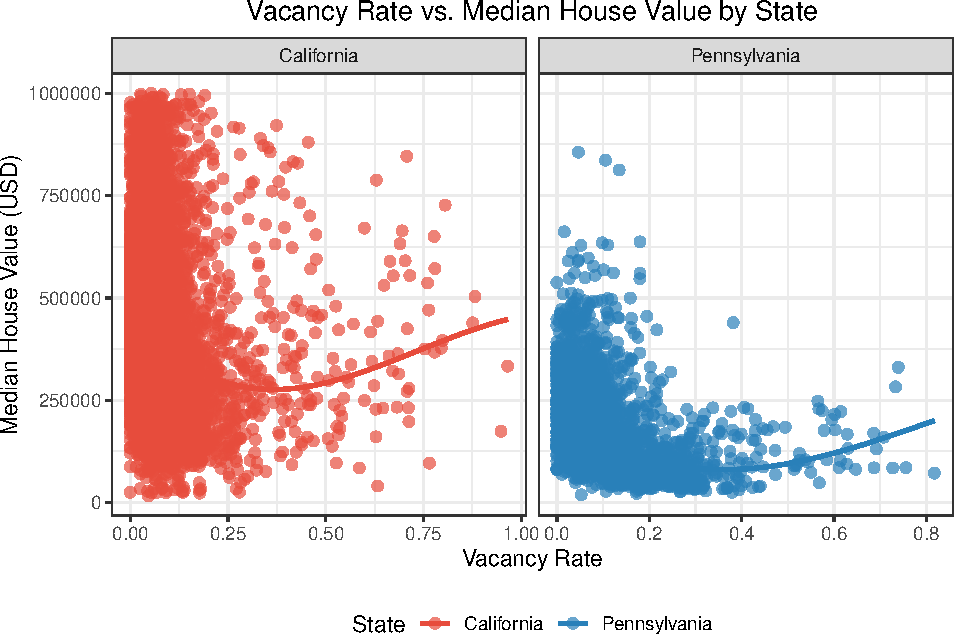
\includegraphics{Homework-02_files/figure-latex/unnamed-chunk-10-1.pdf}

\begin{Shaded}
\begin{Highlighting}[]
\NormalTok{ca\_stats }\OtherTok{\textless{}{-}}\NormalTok{ ca\_pa\_clean }\SpecialCharTok{\%\textgreater{}\%}
  \FunctionTok{filter}\NormalTok{(state }\SpecialCharTok{==} \StringTok{"California"}\NormalTok{) }\SpecialCharTok{\%\textgreater{}\%}
  \FunctionTok{summarise}\NormalTok{(}\AttributeTok{correlation =} \FunctionTok{cor}\NormalTok{(Median\_house\_value, Vacancy\_Rate, }\AttributeTok{use =} \StringTok{"complete.obs"}\NormalTok{))}

\NormalTok{pa\_stats }\OtherTok{\textless{}{-}}\NormalTok{ ca\_pa\_clean }\SpecialCharTok{\%\textgreater{}\%}
  \FunctionTok{filter}\NormalTok{(state }\SpecialCharTok{==} \StringTok{"Pennsylvania"}\NormalTok{) }\SpecialCharTok{\%\textgreater{}\%}
  \FunctionTok{summarise}\NormalTok{(}\AttributeTok{correlation =} \FunctionTok{cor}\NormalTok{(Median\_house\_value, Vacancy\_Rate, }\AttributeTok{use =} \StringTok{"complete.obs"}\NormalTok{))}

\FunctionTok{cat}\NormalTok{(}\StringTok{"}\SpecialCharTok{\textbackslash{}n}\StringTok{差异观察:}\SpecialCharTok{\textbackslash{}n}\StringTok{"}\NormalTok{)}
\end{Highlighting}
\end{Shaded}

\begin{verbatim}
## 
## 差异观察:
\end{verbatim}

\begin{Shaded}
\begin{Highlighting}[]
\FunctionTok{cat}\NormalTok{(}\StringTok{"{-} 加利福尼亚: 房价与空置率相关性:"}\NormalTok{, }\FunctionTok{round}\NormalTok{(ca\_stats}\SpecialCharTok{$}\NormalTok{correlation, }\DecValTok{3}\NormalTok{), }
    \StringTok{"(高房价区域空置率普遍较低,低端市场空置率较高)}\SpecialCharTok{\textbackslash{}n}\StringTok{"}\NormalTok{)}
\end{Highlighting}
\end{Shaded}

\begin{verbatim}
## - 加利福尼亚: 房价与空置率相关性: -0.158 (高房价区域空置率普遍较低,低端市场空置率较高)
\end{verbatim}

\begin{Shaded}
\begin{Highlighting}[]
\FunctionTok{cat}\NormalTok{(}\StringTok{"{-} 宾夕法尼亚: 房价与空置率相关性:"}\NormalTok{, }\FunctionTok{round}\NormalTok{(pa\_stats}\SpecialCharTok{$}\NormalTok{correlation, }\DecValTok{3}\NormalTok{), }
    \StringTok{"(相关性较弱,极端高空置率现象较少)}\SpecialCharTok{\textbackslash{}n}\StringTok{"}\NormalTok{)}
\end{Highlighting}
\end{Shaded}

\begin{verbatim}
## - 宾夕法尼亚: 房价与空置率相关性: -0.336 (相关性较弱,极端高空置率现象较少)
\end{verbatim}

\begin{Shaded}
\begin{Highlighting}[]
\FunctionTok{cat}\NormalTok{(}\StringTok{"{-} 对比: 加州房价对空置率的影响更明显,高端房产市场空置率显著低于宾州"}\NormalTok{)}
\end{Highlighting}
\end{Shaded}

\begin{verbatim}
## - 对比: 加州房价对空置率的影响更明显,高端房产市场空置率显著低于宾州
\end{verbatim}

\subsubsection{4.}\label{section}

The column \texttt{COUNTYFP} contains a numerical code for counties
within each state. We are interested in Alameda County (county 1 in
California), Santa Clara (county 85 in California), and Allegheny County
(county 3 in Pennsylvania).

\paragraph{a.}\label{a.-3}

Explain what the block of code at the end of this question is supposed
to accomplish, and how it does it.

可以用以下代码完成

\begin{Shaded}
\begin{Highlighting}[]
\NormalTok{acca }\OtherTok{\textless{}{-}} \FunctionTok{c}\NormalTok{()}
\ControlFlowTok{for}\NormalTok{ (tract }\ControlFlowTok{in} \DecValTok{1}\SpecialCharTok{:}\FunctionTok{nrow}\NormalTok{(ca\_pa\_clean)) \{}
  \ControlFlowTok{if}\NormalTok{ (ca\_pa}\SpecialCharTok{$}\NormalTok{STATEFP[tract] }\SpecialCharTok{==} \DecValTok{6}\NormalTok{) \{           }\CommentTok{\# 筛选加州(州代码6)}
    \ControlFlowTok{if}\NormalTok{ (ca\_pa}\SpecialCharTok{$}\NormalTok{COUNTYFP[tract] }\SpecialCharTok{==} \DecValTok{1}\NormalTok{) \{        }\CommentTok{\# 筛选阿拉米达县(县代码1)}
\NormalTok{      acca }\OtherTok{\textless{}{-}} \FunctionTok{c}\NormalTok{(acca, tract)                }\CommentTok{\# 记录符合条件的行号}
\NormalTok{    \}}
\NormalTok{  \}}
\NormalTok{\}}
\NormalTok{accamhv }\OtherTok{\textless{}{-}} \FunctionTok{c}\NormalTok{()}
\ControlFlowTok{for}\NormalTok{ (tract }\ControlFlowTok{in}\NormalTok{ acca) \{}
\NormalTok{  accamhv }\OtherTok{\textless{}{-}} \FunctionTok{c}\NormalTok{(accamhv, ca\_pa[tract, }\DecValTok{10}\NormalTok{])    }\CommentTok{\# 提取第10列(房屋价值中位数)}
\NormalTok{\}}
\FunctionTok{median}\NormalTok{(accamhv)                             }\CommentTok{\# 计算所有区的中位数}
\end{Highlighting}
\end{Shaded}

\begin{verbatim}
## [1] NA
\end{verbatim}

\paragraph{b.}\label{b.-3}

Give a single line of R which gives the same final answer as the block
of code. Note: there are at least two ways to do this; you just have to
find one.

可以用以下代码解决

\begin{Shaded}
\begin{Highlighting}[]
\FunctionTok{median}\NormalTok{(ca\_pa}\SpecialCharTok{$}\NormalTok{Median\_house\_value[ca\_pa}\SpecialCharTok{$}\NormalTok{STATEFP }\SpecialCharTok{==} \DecValTok{6} \SpecialCharTok{\&}\NormalTok{ ca\_pa}\SpecialCharTok{$}\NormalTok{COUNTYFP }\SpecialCharTok{==} \DecValTok{1}\NormalTok{], }\AttributeTok{na.rm =} \ConstantTok{TRUE}\NormalTok{)}
\end{Highlighting}
\end{Shaded}

\begin{verbatim}
## [1] 473500
\end{verbatim}

\paragraph{c.}\label{c.-2}

For Alameda, Santa Clara and Allegheny Counties, what were the average
percentages of housing built since 2005?

\begin{Shaded}
\begin{Highlighting}[]
\NormalTok{ca\_pa }\SpecialCharTok{\%\textgreater{}\%}
  \FunctionTok{filter}\NormalTok{(}
\NormalTok{    (STATEFP }\SpecialCharTok{==} \DecValTok{6} \SpecialCharTok{\&}\NormalTok{ COUNTYFP }\SpecialCharTok{==} \DecValTok{1}\NormalTok{) }\SpecialCharTok{|}    \CommentTok{\# Alameda, CA}
\NormalTok{    (STATEFP }\SpecialCharTok{==} \DecValTok{6} \SpecialCharTok{\&}\NormalTok{ COUNTYFP }\SpecialCharTok{==} \DecValTok{85}\NormalTok{) }\SpecialCharTok{|}   \CommentTok{\# Santa Clara, CA}
\NormalTok{    (STATEFP }\SpecialCharTok{==} \DecValTok{42} \SpecialCharTok{\&}\NormalTok{ COUNTYFP }\SpecialCharTok{==} \DecValTok{3}\NormalTok{)     }\CommentTok{\# Allegheny, PA}
\NormalTok{  ) }\SpecialCharTok{\%\textgreater{}\%}
  \FunctionTok{group\_by}\NormalTok{(STATEFP, COUNTYFP) }\SpecialCharTok{\%\textgreater{}\%}
  \FunctionTok{summarise}\NormalTok{(}
    \AttributeTok{Avg\_Percent\_New\_Housing =} \FunctionTok{mean}\NormalTok{(Built\_2005\_or\_later, }\AttributeTok{na.rm =} \ConstantTok{TRUE}\NormalTok{),}
    \AttributeTok{.groups =} \StringTok{"drop"}
\NormalTok{  )}
\end{Highlighting}
\end{Shaded}

\begin{verbatim}
## # A tibble: 3 x 3
##   STATEFP COUNTYFP Avg_Percent_New_Housing
##     <int>    <int>                   <dbl>
## 1       6        1                    2.93
## 2       6       85                    3.16
## 3      42        3                    1.88
\end{verbatim}

\paragraph{d.}\label{d.-1}

The \texttt{cor} function calculates the correlation coefficient between
two variables. What is the correlation between median house value and
the percent of housing built since 2005 in (i) the whole data, (ii) all
of California, (iii) all of Pennsylvania, (iv) Alameda County, (v) Santa
Clara County and (vi) Allegheny County?

\begin{Shaded}
\begin{Highlighting}[]
\NormalTok{cor\_list }\OtherTok{\textless{}{-}} \FunctionTok{list}\NormalTok{(}
  \AttributeTok{whole =} \FunctionTok{cor}\NormalTok{(ca\_pa}\SpecialCharTok{$}\NormalTok{Median\_house\_value, ca\_pa}\SpecialCharTok{$}\NormalTok{Built\_2005\_or\_later, }
              \AttributeTok{use =} \StringTok{"complete.obs"}\NormalTok{),}
  \AttributeTok{california =} \FunctionTok{cor}\NormalTok{(ca\_pa}\SpecialCharTok{$}\NormalTok{Median\_house\_value[ca\_pa}\SpecialCharTok{$}\NormalTok{STATEFP}\SpecialCharTok{==}\DecValTok{6}\NormalTok{], }
\NormalTok{                   ca\_pa}\SpecialCharTok{$}\NormalTok{Built\_2005\_or\_later[ca\_pa}\SpecialCharTok{$}\NormalTok{STATEFP}\SpecialCharTok{==}\DecValTok{6}\NormalTok{], }\AttributeTok{use =} \StringTok{"complete.obs"}\NormalTok{),}
  \AttributeTok{pennsylvania =} \FunctionTok{cor}\NormalTok{(ca\_pa}\SpecialCharTok{$}\NormalTok{Median\_house\_value[ca\_pa}\SpecialCharTok{$}\NormalTok{STATEFP}\SpecialCharTok{==}\DecValTok{42}\NormalTok{], }
\NormalTok{                     ca\_pa}\SpecialCharTok{$}\NormalTok{Built\_2005\_or\_later[ca\_pa}\SpecialCharTok{$}\NormalTok{STATEFP}\SpecialCharTok{==}\DecValTok{42}\NormalTok{], }
\NormalTok{                     use}
                     \OtherTok{=} \StringTok{"complete.obs"}\NormalTok{),}
  \AttributeTok{alameda =} \FunctionTok{cor}\NormalTok{(ca\_pa}\SpecialCharTok{$}\NormalTok{Median\_house\_value[ca\_pa}\SpecialCharTok{$}\NormalTok{COUNTYFP}\SpecialCharTok{==}\DecValTok{1}\NormalTok{], }
\NormalTok{                ca\_pa}\SpecialCharTok{$}\NormalTok{Built\_2005\_or\_later[ca\_pa}\SpecialCharTok{$}\NormalTok{COUNTYFP}\SpecialCharTok{==}\DecValTok{1}\NormalTok{], }
                \AttributeTok{use =} \StringTok{"complete.obs"}\NormalTok{),}
  \AttributeTok{santa\_clara =} \FunctionTok{cor}\NormalTok{(ca\_pa}\SpecialCharTok{$}\NormalTok{Median\_house\_value[ca\_pa}\SpecialCharTok{$}\NormalTok{COUNTYFP}\SpecialCharTok{==}\DecValTok{85}\NormalTok{],}
\NormalTok{                    ca\_pa}\SpecialCharTok{$}\NormalTok{Built\_2005\_or\_later[ca\_pa}\SpecialCharTok{$}\NormalTok{COUNTYFP}\SpecialCharTok{==}\DecValTok{85}\NormalTok{], }
                    \AttributeTok{use =} \StringTok{"complete.obs"}\NormalTok{),}
  \AttributeTok{allegheny =} \FunctionTok{cor}\NormalTok{(ca\_pa}\SpecialCharTok{$}\NormalTok{Median\_house\_value[ca\_pa}\SpecialCharTok{$}\NormalTok{COUNTYFP}\SpecialCharTok{==}\DecValTok{3}\NormalTok{], }
\NormalTok{                  ca\_pa}\SpecialCharTok{$}\NormalTok{Built\_2005\_or\_later[ca\_pa}\SpecialCharTok{$}\NormalTok{COUNTYFP}\SpecialCharTok{==}\DecValTok{3}\NormalTok{], }\AttributeTok{use =} \StringTok{"complete.obs"}\NormalTok{)}
\NormalTok{)}
\FunctionTok{print}\NormalTok{(cor\_list)}
\end{Highlighting}
\end{Shaded}

\begin{verbatim}
## $whole
## [1] -0.02052684
## 
## $california
## [1] -0.1160322
## 
## $pennsylvania
## [1] 0.2339447
## 
## $alameda
## [1] -0.0357215
## 
## $santa_clara
## [1] -0.08501218
## 
## $allegheny
## [1] 0.1846541
\end{verbatim}

\paragraph{e.}\label{e.-1}

Make three plots, showing median house values against median income, for
Alameda, Santa Clara, and Allegheny Counties. (If you can fit the
information into one plot, clearly distinguishing the three counties,
that's OK too.)、

\begin{Shaded}
\begin{Highlighting}[]
\FunctionTok{library}\NormalTok{(ggplot2)}
\NormalTok{ca\_pa }\SpecialCharTok{\%\textgreater{}\%}
  \FunctionTok{filter}\NormalTok{(COUNTYFP }\SpecialCharTok{\%in\%} \FunctionTok{c}\NormalTok{(}\DecValTok{1}\NormalTok{, }\DecValTok{85}\NormalTok{, }\DecValTok{3}\NormalTok{)) }\SpecialCharTok{\%\textgreater{}\%}
  \FunctionTok{mutate}\NormalTok{(}\AttributeTok{County =} \FunctionTok{case\_when}\NormalTok{(}
\NormalTok{    COUNTYFP }\SpecialCharTok{==} \DecValTok{1} \SpecialCharTok{\textasciitilde{}} \StringTok{"Alameda"}\NormalTok{,}
\NormalTok{    COUNTYFP }\SpecialCharTok{==} \DecValTok{85} \SpecialCharTok{\textasciitilde{}} \StringTok{"Santa Clara"}\NormalTok{,}
\NormalTok{    COUNTYFP }\SpecialCharTok{==} \DecValTok{3} \SpecialCharTok{\textasciitilde{}} \StringTok{"Allegheny"}
\NormalTok{  )) }\SpecialCharTok{\%\textgreater{}\%}
  \FunctionTok{ggplot}\NormalTok{(}\FunctionTok{aes}\NormalTok{(}\AttributeTok{x =}\NormalTok{ Median\_household\_income, }\AttributeTok{y =}\NormalTok{ Median\_house\_value, }\AttributeTok{color =}\NormalTok{ County)) }\SpecialCharTok{+}
  \FunctionTok{geom\_point}\NormalTok{(}\AttributeTok{alpha =} \FloatTok{0.7}\NormalTok{, }\AttributeTok{size =} \DecValTok{2}\NormalTok{) }\SpecialCharTok{+}
  \FunctionTok{geom\_smooth}\NormalTok{(}\AttributeTok{method =} \StringTok{"lm"}\NormalTok{, }\AttributeTok{se =} \ConstantTok{FALSE}\NormalTok{) }\SpecialCharTok{+}
  \FunctionTok{scale\_y\_continuous}\NormalTok{(}\AttributeTok{labels =}\NormalTok{ scales}\SpecialCharTok{::}\NormalTok{dollar) }\SpecialCharTok{+}
  \FunctionTok{scale\_x\_continuous}\NormalTok{(}\AttributeTok{labels =}\NormalTok{ scales}\SpecialCharTok{::}\NormalTok{dollar) }\SpecialCharTok{+}
  \FunctionTok{labs}\NormalTok{(}
    \AttributeTok{title =} \StringTok{"The Relationship Between Housing Value and Household Income"}\NormalTok{,}
    \AttributeTok{x =} \StringTok{"Median household income"}\NormalTok{,}
    \AttributeTok{y =} \StringTok{"Median home value"}\NormalTok{,}
    \AttributeTok{color =} \StringTok{"County"}
\NormalTok{  ) }\SpecialCharTok{+}
  \FunctionTok{theme\_minimal}\NormalTok{() }\SpecialCharTok{+}
  \FunctionTok{scale\_color\_manual}\NormalTok{(}\AttributeTok{values =} \FunctionTok{c}\NormalTok{(}\StringTok{"Alameda"} \OtherTok{=} \StringTok{"\#E41A1C"}\NormalTok{, }
                               \StringTok{"Santa Clara"} \OtherTok{=} \StringTok{"\#377EB8"}\NormalTok{,}
                               \StringTok{"Allegheny"} \OtherTok{=} \StringTok{"\#4DAF4A"}\NormalTok{))}
\end{Highlighting}
\end{Shaded}

\begin{verbatim}
## `geom_smooth()` using formula = 'y ~ x'
\end{verbatim}

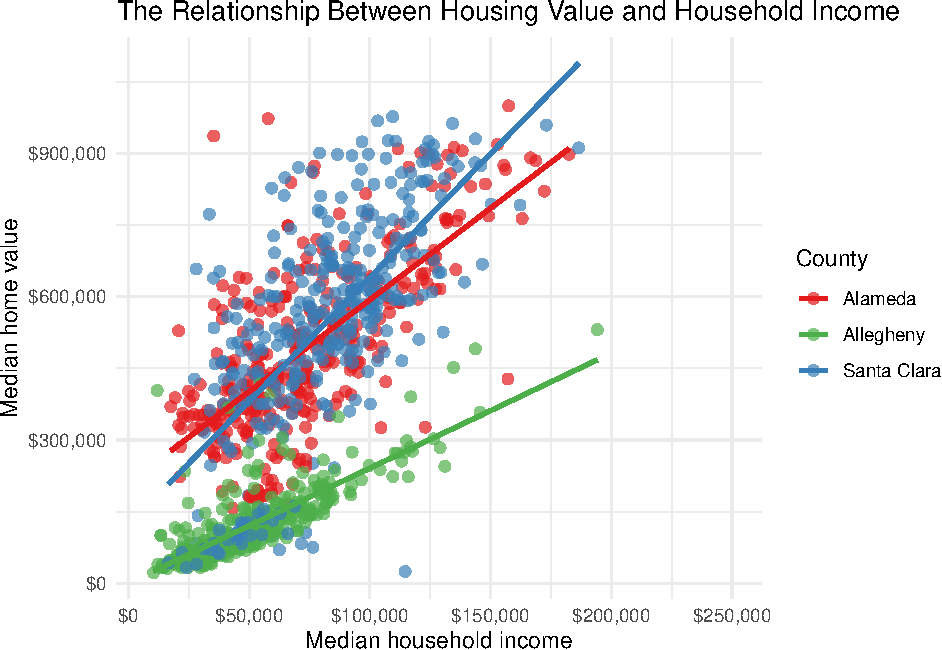
\includegraphics{Homework-02_files/figure-latex/unnamed-chunk-15-1.pdf}

\subsubsection{MB.Ch1.11.}\label{mb.ch1.11.}

Run the following code.Explain the output from the successive uses of
table().

创建了一个包含91个''female''和92个''male''的因子向量
默认情况下:水平(levels)按字母顺序排序:``female''在前,``male''在后,table()统计了每个水平的真实数量.

\begin{Shaded}
\begin{Highlighting}[]
\NormalTok{gender }\OtherTok{\textless{}{-}} \FunctionTok{factor}\NormalTok{(}\FunctionTok{c}\NormalTok{(}\FunctionTok{rep}\NormalTok{(}\StringTok{"female"}\NormalTok{, }\DecValTok{91}\NormalTok{), }\FunctionTok{rep}\NormalTok{(}\StringTok{"male"}\NormalTok{, }\DecValTok{92}\NormalTok{)))}
\FunctionTok{table}\NormalTok{(gender)}
\end{Highlighting}
\end{Shaded}

\begin{verbatim}
## gender
## female   male 
##     91     92
\end{verbatim}

使用levels参数显式指定新顺序:``male''在前,``female''在后
table()输出:遵循新的水平顺序(先显示''male''),统计数量不变,但顺序改变了

\begin{Shaded}
\begin{Highlighting}[]
\NormalTok{gender }\OtherTok{\textless{}{-}} \FunctionTok{factor}\NormalTok{(gender, }\AttributeTok{levels=}\FunctionTok{c}\NormalTok{(}\StringTok{"male"}\NormalTok{, }\StringTok{"female"}\NormalTok{))}
\FunctionTok{table}\NormalTok{(gender)}
\end{Highlighting}
\end{Shaded}

\begin{verbatim}
## gender
##   male female 
##     92     91
\end{verbatim}

将''male''改为''Male'' 所有原''male''值(92个)不匹配新水平,转为NA
原''female''值(91个)匹配新水平''female''
新水平''Male''无匹配数据,显示为0

\begin{Shaded}
\begin{Highlighting}[]
\NormalTok{gender }\OtherTok{\textless{}{-}} \FunctionTok{factor}\NormalTok{(gender, }\AttributeTok{levels=}\FunctionTok{c}\NormalTok{(}\StringTok{"Male"}\NormalTok{, }\StringTok{"female"}\NormalTok{))}
\CommentTok{\# Note the mistake: "Male" should be "male"}
\FunctionTok{table}\NormalTok{(gender)}
\end{Highlighting}
\end{Shaded}

\begin{verbatim}
## gender
##   Male female 
##      0     91
\end{verbatim}

exclude=NULL参数:强制包含所有NA值 输出包含三个部分:
``Male'':无匹配数据(0个) ``female'':原female值(91个)
:原male值转换的缺失值(92个)

\begin{Shaded}
\begin{Highlighting}[]
\FunctionTok{table}\NormalTok{(gender, }\AttributeTok{exclude=}\ConstantTok{NULL}\NormalTok{)}
\end{Highlighting}
\end{Shaded}

\begin{verbatim}
## gender
##   Male female   <NA> 
##      0     91     92
\end{verbatim}

清除gender

\begin{Shaded}
\begin{Highlighting}[]
\FunctionTok{rm}\NormalTok{(gender)  }\CommentTok{\# Remove gender}
\end{Highlighting}
\end{Shaded}

\subsubsection{MB.Ch1.12.}\label{mb.ch1.12.}

Write a function that calculates the proportion of values in a vector x
that exceed some value cutoff.

\begin{Shaded}
\begin{Highlighting}[]
\CommentTok{\#\textquotesingle{} @param x 输入数值向量}
\CommentTok{\#\textquotesingle{} @@param cutoff 截止值}
\CommentTok{\#\textquotesingle{} @return 超过截止值的元素比例}
\NormalTok{exceeding\_proportion }\OtherTok{\textless{}{-}} \ControlFlowTok{function}\NormalTok{(x, cutoff) \{}
  \ControlFlowTok{if}\NormalTok{ (}\FunctionTok{length}\NormalTok{(x) }\SpecialCharTok{==} \DecValTok{0}\NormalTok{) }\FunctionTok{return}\NormalTok{(}\DecValTok{0}\NormalTok{)  }\CommentTok{\# 处理空向量情况}
  \FunctionTok{sum}\NormalTok{(x }\SpecialCharTok{\textgreater{}}\NormalTok{ cutoff) }\SpecialCharTok{/} \FunctionTok{length}\NormalTok{(x)}
\NormalTok{\}}
\end{Highlighting}
\end{Shaded}

\paragraph{(a)}\label{a}

Use the sequence of numbers 1, 2, . . . , 100 to check that this
function gives the result that is expected.

\begin{Shaded}
\begin{Highlighting}[]
\CommentTok{\# 测试各种截止值情况}
\NormalTok{test\_vector }\OtherTok{\textless{}{-}} \DecValTok{1}\SpecialCharTok{:}\DecValTok{100}

\CommentTok{\# 当截止值=0(所有元素)}
\FunctionTok{exceeding\_proportion}\NormalTok{(test\_vector, }\DecValTok{0}\NormalTok{)   }\CommentTok{\# 预期: 1.0}
\end{Highlighting}
\end{Shaded}

\begin{verbatim}
## [1] 1
\end{verbatim}

\begin{Shaded}
\begin{Highlighting}[]
\CommentTok{\# 当截止值=50(50个元素)}
\FunctionTok{exceeding\_proportion}\NormalTok{(test\_vector, }\DecValTok{50}\NormalTok{)  }\CommentTok{\# 预期: 0.5}
\end{Highlighting}
\end{Shaded}

\begin{verbatim}
## [1] 0.5
\end{verbatim}

\begin{Shaded}
\begin{Highlighting}[]
\CommentTok{\# 当截止值=100(无元素)}
\FunctionTok{exceeding\_proportion}\NormalTok{(test\_vector, }\DecValTok{100}\NormalTok{) }\CommentTok{\# 预期: 0.0}
\end{Highlighting}
\end{Shaded}

\begin{verbatim}
## [1] 0
\end{verbatim}

\begin{Shaded}
\begin{Highlighting}[]
\CommentTok{\# 当截止值=101(无元素)}
\FunctionTok{exceeding\_proportion}\NormalTok{(test\_vector, }\DecValTok{101}\NormalTok{) }\CommentTok{\# 预期: 0.0}
\end{Highlighting}
\end{Shaded}

\begin{verbatim}
## [1] 0
\end{verbatim}

\begin{Shaded}
\begin{Highlighting}[]
\CommentTok{\# 边缘情况测试}
\FunctionTok{exceeding\_proportion}\NormalTok{(}\FunctionTok{numeric}\NormalTok{(}\DecValTok{0}\NormalTok{), }\DecValTok{5}\NormalTok{)    }\CommentTok{\# 空向量返回0}
\end{Highlighting}
\end{Shaded}

\begin{verbatim}
## [1] 0
\end{verbatim}

\begin{Shaded}
\begin{Highlighting}[]
\FunctionTok{exceeding\_proportion}\NormalTok{(}\FunctionTok{c}\NormalTok{(}\DecValTok{5}\NormalTok{, }\DecValTok{5}\NormalTok{, }\DecValTok{5}\NormalTok{), }\DecValTok{5}\NormalTok{)    }\CommentTok{\# 严格大于,返回0}
\end{Highlighting}
\end{Shaded}

\begin{verbatim}
## [1] 0
\end{verbatim}

\paragraph{(b)}\label{b}

Obtain the vector ex01.36 from the Devore6 (or Devore7) package. These
data give the times required for individuals to escape from an oil
platform during a drill. Use dotplot() to show the distribution of
times. Calculate the proportion of escape times that exceed 7 minutes.

\begin{Shaded}
\begin{Highlighting}[]
\FunctionTok{library}\NormalTok{(Devore7)}
\FunctionTok{data}\NormalTok{(}\StringTok{"ex01.36"}\NormalTok{, }\AttributeTok{package =} \StringTok{"Devore7"}\NormalTok{)}
\NormalTok{escape\_times\_seconds }\OtherTok{\textless{}{-}}\NormalTok{ ex01}\FloatTok{.36}\NormalTok{[[}\DecValTok{1}\NormalTok{]]}

\NormalTok{cutoff\_seconds }\OtherTok{\textless{}{-}} \DecValTok{420}  \CommentTok{\# 7分钟转换为秒}

\CommentTok{\# 计算超过420秒的比例}
\NormalTok{prop\_over\_420sec }\OtherTok{\textless{}{-}} \FunctionTok{exceeding\_proportion}\NormalTok{(escape\_times\_seconds, cutoff\_seconds)}
\NormalTok{count\_above }\OtherTok{\textless{}{-}} \FunctionTok{sum}\NormalTok{(escape\_times\_seconds }\SpecialCharTok{\textgreater{}}\NormalTok{ cutoff\_seconds)}
\NormalTok{n\_total }\OtherTok{\textless{}{-}} \FunctionTok{length}\NormalTok{(escape\_times\_seconds)}

\FunctionTok{cat}\NormalTok{(}\StringTok{"撤离时间分析结果 (秒单位):}\SpecialCharTok{\textbackslash{}n}\StringTok{"}\NormalTok{)}
\end{Highlighting}
\end{Shaded}

\begin{verbatim}
## 撤离时间分析结果 (秒单位):
\end{verbatim}

\begin{Shaded}
\begin{Highlighting}[]
\FunctionTok{cat}\NormalTok{(}\StringTok{"总观测数:"}\NormalTok{, n\_total, }\StringTok{"}\SpecialCharTok{\textbackslash{}n}\StringTok{"}\NormalTok{)}
\end{Highlighting}
\end{Shaded}

\begin{verbatim}
## 总观测数: 26
\end{verbatim}

\begin{Shaded}
\begin{Highlighting}[]
\FunctionTok{cat}\NormalTok{(}\StringTok{"超过420秒的观测数:"}\NormalTok{, count\_above, }\StringTok{"}\SpecialCharTok{\textbackslash{}n}\StringTok{"}\NormalTok{)}
\end{Highlighting}
\end{Shaded}

\begin{verbatim}
## 超过420秒的观测数: 1
\end{verbatim}

\begin{Shaded}
\begin{Highlighting}[]
\FunctionTok{cat}\NormalTok{(}\StringTok{"超过420秒的比例:"}\NormalTok{, }\FunctionTok{round}\NormalTok{(prop\_over\_420sec, }\DecValTok{4}\NormalTok{), }\StringTok{"}\SpecialCharTok{\textbackslash{}n}\StringTok{"}\NormalTok{)}
\end{Highlighting}
\end{Shaded}

\begin{verbatim}
## 超过420秒的比例: 0.0385
\end{verbatim}

\begin{Shaded}
\begin{Highlighting}[]
\FunctionTok{cat}\NormalTok{(}\StringTok{"分数表示:"}\NormalTok{, count\_above, }\StringTok{"/"}\NormalTok{, n\_total, }\StringTok{"}\SpecialCharTok{\textbackslash{}n\textbackslash{}n}\StringTok{"}\NormalTok{)}
\end{Highlighting}
\end{Shaded}

\begin{verbatim}
## 分数表示: 1 / 26
\end{verbatim}

\begin{Shaded}
\begin{Highlighting}[]
\NormalTok{custom\_dotplot }\OtherTok{\textless{}{-}} \ControlFlowTok{function}\NormalTok{(x, cutoff, }\AttributeTok{unit =} \StringTok{"seconds"}\NormalTok{) \{}

\NormalTok{  unique\_vals }\OtherTok{\textless{}{-}} \FunctionTok{sort}\NormalTok{(}\FunctionTok{unique}\NormalTok{(}\FunctionTok{round}\NormalTok{(x, }\DecValTok{2}\NormalTok{)))}
\NormalTok{  y\_pos }\OtherTok{\textless{}{-}} \FunctionTok{seq\_along}\NormalTok{(unique\_vals)}
  
\NormalTok{  y\_vals }\OtherTok{\textless{}{-}} \FunctionTok{sapply}\NormalTok{(x, }\ControlFlowTok{function}\NormalTok{(val) \{}
\NormalTok{    match\_idx }\OtherTok{\textless{}{-}} \FunctionTok{which.min}\NormalTok{(}\FunctionTok{abs}\NormalTok{(unique\_vals }\SpecialCharTok{{-}}\NormalTok{ val))}
\NormalTok{    y\_pos[match\_idx]}
\NormalTok{  \})}

  \FunctionTok{plot}\NormalTok{(}\DecValTok{1}\NormalTok{, }\AttributeTok{type =} \StringTok{"n"}\NormalTok{, }
       \AttributeTok{xlim =} \FunctionTok{range}\NormalTok{(x), }
       \AttributeTok{ylim =} \FunctionTok{c}\NormalTok{(}\DecValTok{0}\NormalTok{, }\FunctionTok{max}\NormalTok{(y\_pos) }\SpecialCharTok{+} \DecValTok{1}\NormalTok{),}
       \AttributeTok{main =} \StringTok{"Distribution of Escape Times"}\NormalTok{,}
       \AttributeTok{xlab =} \FunctionTok{paste}\NormalTok{(}\StringTok{"Escape Time ("}\NormalTok{, unit, }\StringTok{")"}\NormalTok{, }\AttributeTok{sep =} \StringTok{""}\NormalTok{),}
       \AttributeTok{ylab =} \StringTok{"Count"}\NormalTok{, }\AttributeTok{yaxt =} \StringTok{"n"}\NormalTok{)}
  
  \FunctionTok{points}\NormalTok{(x, y\_vals, }\AttributeTok{pch =} \DecValTok{16}\NormalTok{, }\AttributeTok{col =} \StringTok{"steelblue"}\NormalTok{)}
  
  \FunctionTok{abline}\NormalTok{(}\AttributeTok{v =}\NormalTok{ cutoff, }\AttributeTok{col =} \StringTok{"red"}\NormalTok{, }\AttributeTok{lty =} \DecValTok{2}\NormalTok{, }\AttributeTok{lwd =} \DecValTok{2}\NormalTok{)}
  
\NormalTok{\}}
\FunctionTok{custom\_dotplot}\NormalTok{(escape\_times\_seconds, cutoff\_seconds, }\StringTok{"seconds"}\NormalTok{)}
\end{Highlighting}
\end{Shaded}

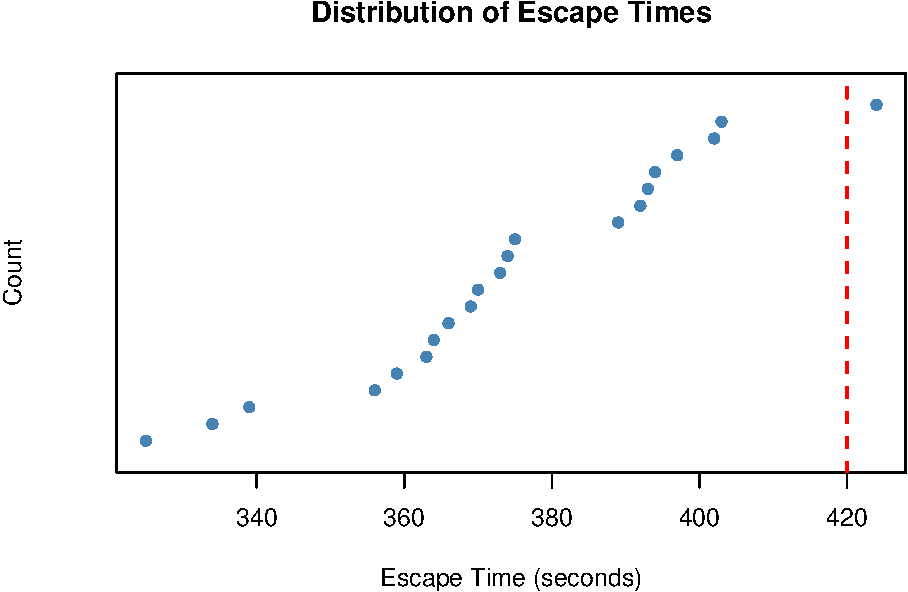
\includegraphics{Homework-02_files/figure-latex/unnamed-chunk-23-1.pdf}

\subsubsection{MB.Ch1.18.}\label{mb.ch1.18.}

The Rabbit data frame in the MASS library contains blood pressure change
measurements on five rabbits (labeled as R1, R2, . . . ,R5) under
various control and treatment conditions. Read the help file for more
information. Use the unstack() function (three times) to convert Rabbit
to the following form:

Treatment Dose R1 R2 R3 R4 R5

1 Control 6.25 0.50 1.00 0.75 1.25 1.5

2 Control 12.50 4.50 1.25 3.00 1.50 1.5

\ldots.

\begin{Shaded}
\begin{Highlighting}[]
\FunctionTok{library}\NormalTok{(MASS)}

\NormalTok{final\_result }\OtherTok{\textless{}{-}} \FunctionTok{aggregate}\NormalTok{(BPchange }\SpecialCharTok{\textasciitilde{}}\NormalTok{ Treatment }\SpecialCharTok{+}\NormalTok{ Dose }\SpecialCharTok{+}\NormalTok{ Animal, }\AttributeTok{data =}\NormalTok{ Rabbit, }\AttributeTok{FUN =}\NormalTok{ mean)}

\NormalTok{final\_result\_wide }\OtherTok{\textless{}{-}} \FunctionTok{reshape}\NormalTok{(final\_result,}
                           \AttributeTok{timevar =} \StringTok{"Animal"}\NormalTok{,}
                           \AttributeTok{idvar =} \FunctionTok{c}\NormalTok{(}\StringTok{"Treatment"}\NormalTok{, }\StringTok{"Dose"}\NormalTok{),}
                           \AttributeTok{direction =} \StringTok{"wide"}\NormalTok{)}

\NormalTok{rabbit\_cols }\OtherTok{\textless{}{-}} \FunctionTok{grep}\NormalTok{(}\StringTok{"BPchange."}\NormalTok{, }\FunctionTok{colnames}\NormalTok{(final\_result\_wide), }\AttributeTok{value =} \ConstantTok{TRUE}\NormalTok{)}
\NormalTok{rabbit\_names }\OtherTok{\textless{}{-}} \FunctionTok{gsub}\NormalTok{(}\StringTok{"BPchange."}\NormalTok{, }\StringTok{""}\NormalTok{, rabbit\_cols)}

\NormalTok{required\_columns }\OtherTok{\textless{}{-}} \FunctionTok{c}\NormalTok{(}\StringTok{"Treatment"}\NormalTok{, }\StringTok{"Dose"}\NormalTok{, rabbit\_cols)}
\NormalTok{final\_result\_wide }\OtherTok{\textless{}{-}}\NormalTok{ final\_result\_wide[, required\_columns]}

\FunctionTok{colnames}\NormalTok{(final\_result\_wide) }\OtherTok{\textless{}{-}} \FunctionTok{c}\NormalTok{(}\StringTok{"Treatment"}\NormalTok{, }\StringTok{"Dose"}\NormalTok{, rabbit\_names)}

\NormalTok{final\_result\_wide }\OtherTok{\textless{}{-}}\NormalTok{ final\_result\_wide[}\FunctionTok{order}\NormalTok{(final\_result\_wide}\SpecialCharTok{$}\NormalTok{Treatment), ]}

\FunctionTok{print}\NormalTok{(final\_result\_wide)}
\end{Highlighting}
\end{Shaded}

\begin{verbatim}
##    Treatment   Dose    R1    R2    R3    R4   R5
## 1    Control   6.25  0.50  1.00  0.75  1.25  1.5
## 3    Control  12.50  4.50  1.25  3.00  1.50  1.5
## 5    Control  25.00 10.00  4.00  3.00  6.00  5.0
## 7    Control  50.00 26.00 12.00 14.00 19.00 16.0
## 9    Control 100.00 37.00 27.00 22.00 33.00 20.0
## 11   Control 200.00 32.00 29.00 24.00 33.00 18.0
## 2        MDL   6.25  1.25  1.40  0.75  2.60  2.4
## 4        MDL  12.50  0.75  1.70  2.30  1.20  2.5
## 6        MDL  25.00  4.00  1.00  3.00  2.00  1.5
## 8        MDL  50.00  9.00  2.00  5.00  3.00  2.0
## 10       MDL 100.00 25.00 15.00 26.00 11.00  9.0
## 12       MDL 200.00 37.00 28.00 25.00 22.00 19.0
\end{verbatim}

\end{document}
